\subsection{Use Case: Numeric Weather Prediction}

\paragraph*{Background.}

Large amounts of weather data ar e produced continually and stored in
many different databases.  Accurate weather predictions require large
amount s of processing power to accurately simulate conditions
worldwide at a high resolution and fre quent intervals. One of the
most computationally consuming parts of a reliable weather model is th
e microphysics scheme. The current microphysics scheme, Weather
Research and Forecasting (WRF) Single Moment 6-class Microphysics
(WSM6), simulates the processes in the atmosphere that leadto the
formation and precipitation of rain, snow, and graupel and requires
complex floating-point operations needing to be performed on vast
amounts of data for accurate simulations. As computer
performanceimproves, so does the Numerical Weather Prediction (NWP)
models' resolution and accuracy. However, there is still much progress
to be made, as simulation accuracy still falls off sign ificantly for
predictions more than 36 hours in advance. Figure \ref{fig:weather-1}
shows the general WRF modeling system flow chat.

\begin{figure}[htb]
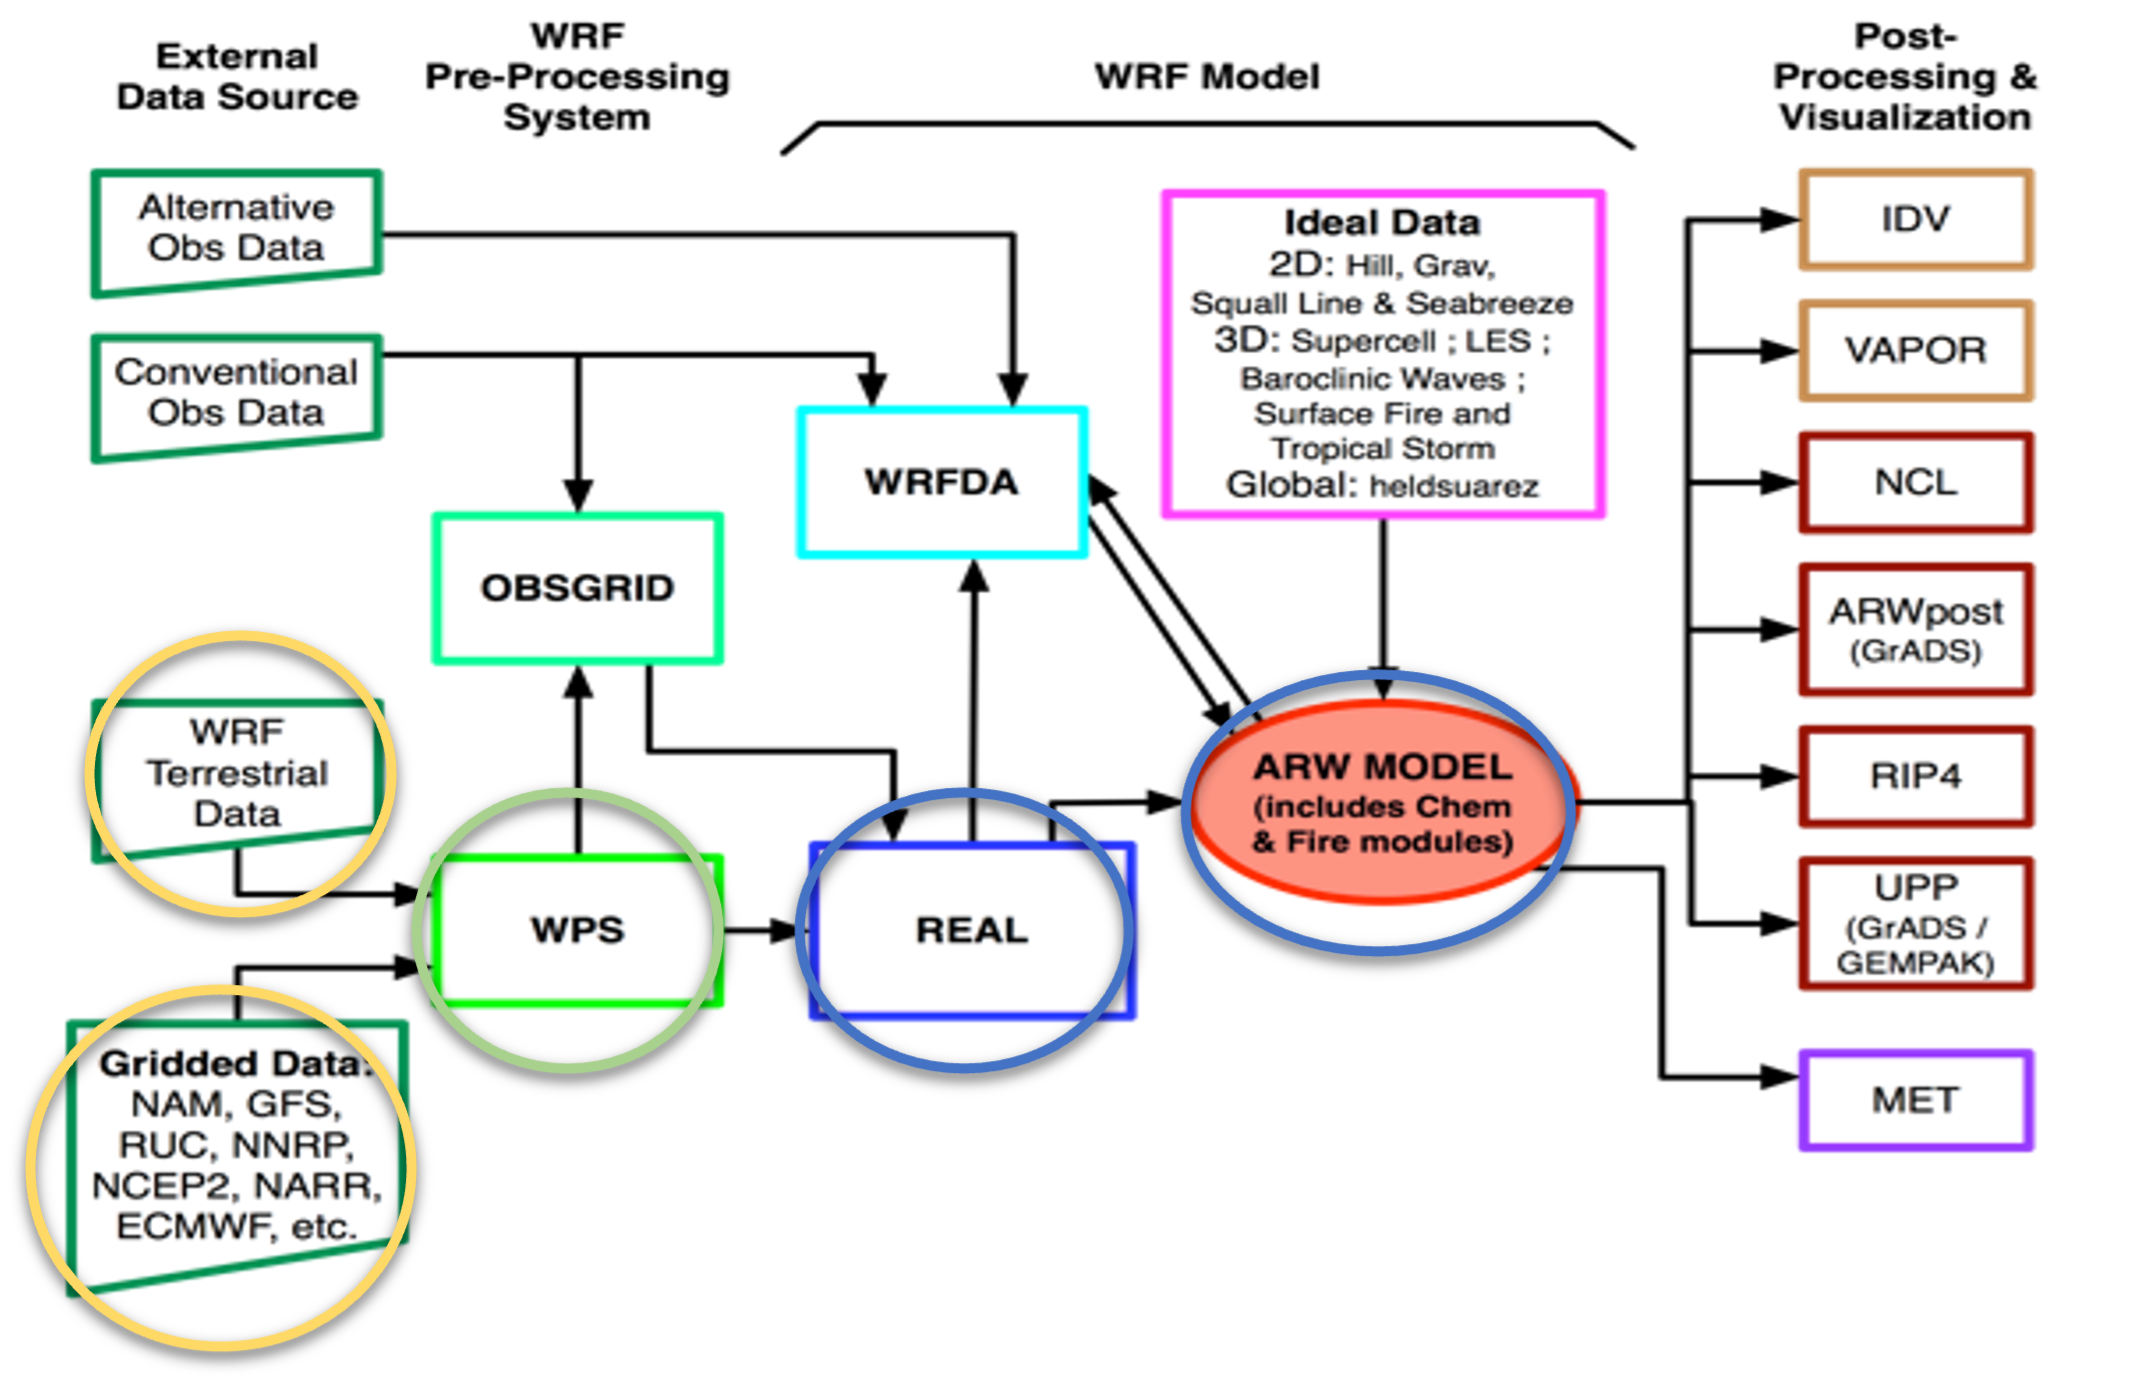
\includegraphics[width=1.0\textwidth]{usecase/nwp-arch.png}
\label{fig:weather-1}
\caption{WRF Modeling System Flow Chart with Various Configuration.}
\end{figure}


\paragraph*{Functionalities and Activities} (based on Big Data Application Provider of NBDIF Ref. Architecture).
In this case study, we only focus on two main functionalities, namely
WPS and WRF, and their activities.  Figure \ref{fig:weather-2} shows
the cross-functional diagram for their actions.

WPS Activities:

\begin{figure}[htb]
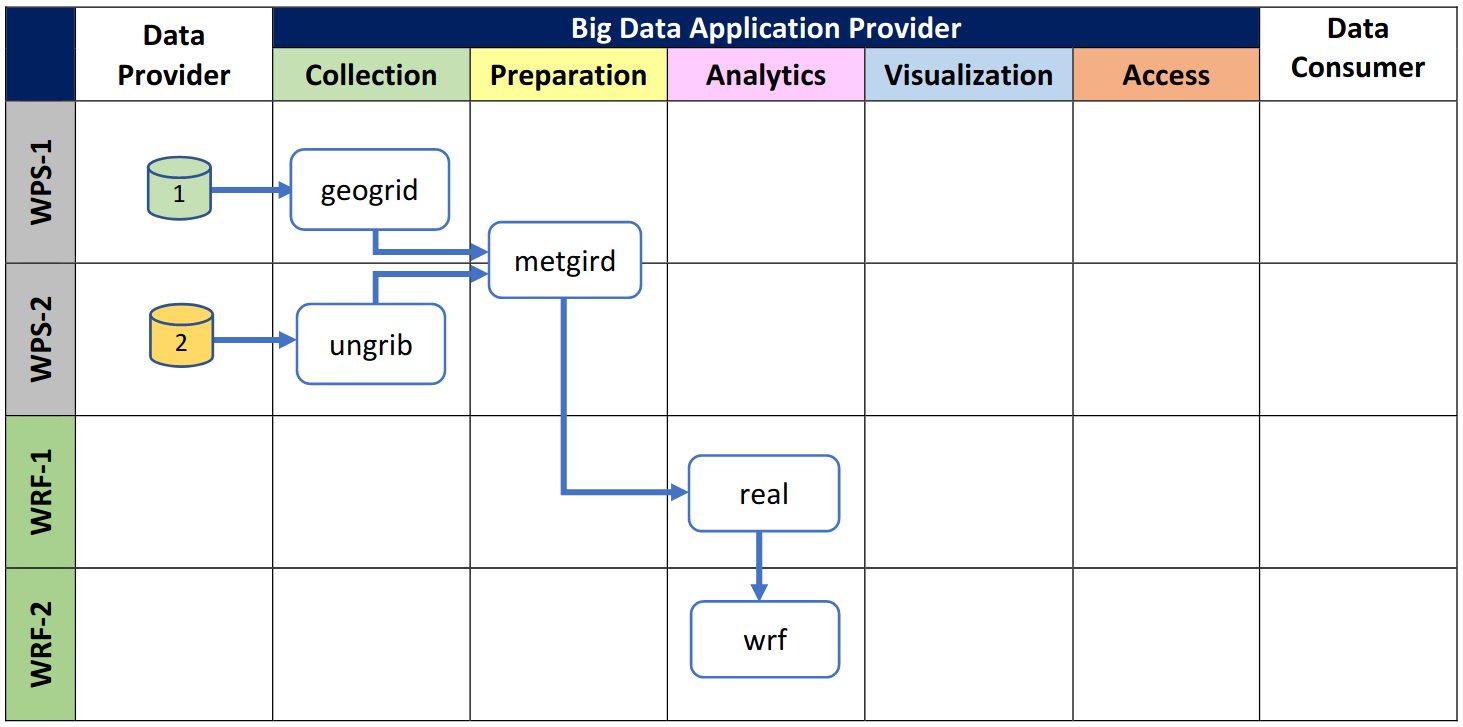
\includegraphics[width=1.0\textwidth]{usecase/weather.png}
\label{fig:weather-2}
\caption{Cross-Functional Diagram Numerical Weather Prediction.}
\end{figure}

\begin{enumerate}
  
\item geogrid – defines simulation domains and interpolate various terrestrial data sets to the
model grids. Input data available at [1].

\item ungrib – extracts needed meteorological data and packs it into an intermediate file format.
Input data available at [2]

\item medgrid – prepares horizontally interpolate the meteorological data onto the model domain.
  Input data from the output of geogrid and ungrib.

\end{enumerate}

WRF Activities:

\begin{enumerate}

\item real – prepares vertically interpolates the output from metgrid, and creates a boundary and initial
condition files with some consistency checks.

\item wrf – generates a model forecast.

\end{enumerate}

\paragraph*{Datasets.}

\begin{enumerate}
  
\item WRF Users Page, WPS V4 Geographical Static Data Downloads Page \cite{wrf-data}

\item NCEP FNL Operational Model Global Tropospheric Analyses, continuing
from July 1999 \cite{cisl_rda_ds083.2}

\end{enumerate}
